%versi 3 (22-07-2020)
\chapter{Landasan Teori}
\label{chap:teori}

\section{Strategy Pattern}
\label{sec:strategypattern}
Strategy Pattern adalah sebuah design pattern yang memungkinkan objek untuk memilih saat runtime. Ini mendefinisikan sekumpulan algoritma, merangkum masing-masing algoritma, dan membuatnya dapat dipertukarkan. Hal ini memungkinkan klien untuk memilih algoritma berdasarkan kebutuhan mereka tanpa mengubah kode yang menggunakan algoritma tersebut. Ide utama penerapan Strategy Pattern adalah merancang antarmuka fleksibel yang dapat bekerja dengan algoritma berbeda tanpa perlu mengubah kode ketika algoritma baru diperkenalkan. \\
Strategy Pattern cocok digunakan dalam skenario-skenario berikut:
\begin{enumerate}
    \item Ketika ada beberapa kelas terkait yang hanya berbeda dalam perilakunya. Strategy Pattern memungkinkan kelas dikonfigurasikan dengan salah satu dari banyak kemungkinan perilaku.
    \item Ketika ada kebutuhan untuk varian algoritma yang berbeda.
    \item Ketika suatu algoritma melibatkan data yang harus tetap tersembunyi dari klien. Strategy Pattern memastikan bahwa struktur data yang kompleks dan spesifik algoritma tidak terekspos.
    \item Ketika sebuah kelas mendefinisikan banyak perilaku, dan perilaku ini diimplementasikan melalui beberapa pernyataan kondisional. Dalam kasus seperti ini, Strategy Pattern menyederhanakan kode dengan memindahkan cabang kondisional terkait ke dalam kelas Strategi masing-masing
\end{enumerate}
\begin{figure}[h] 
	\centering  
	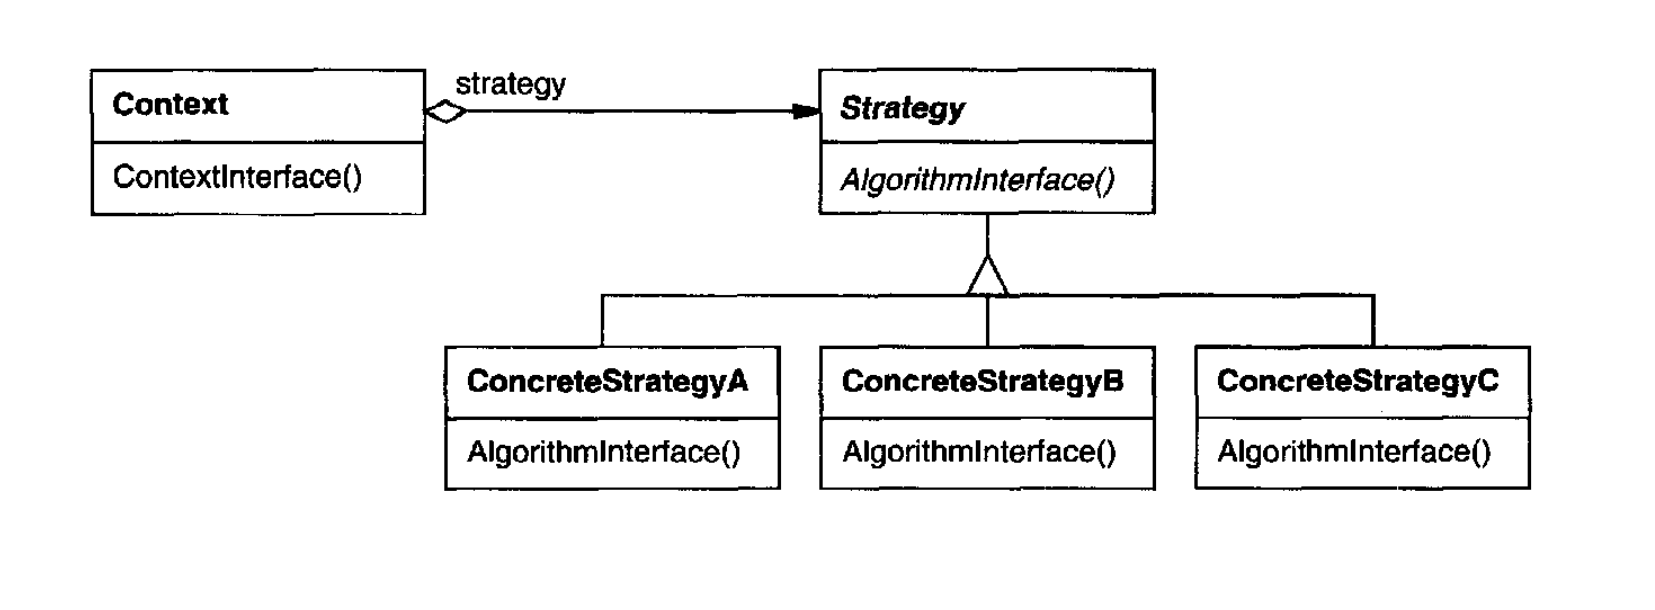
\includegraphics[width=1\textwidth]{struktur-sp}  
	\caption{Struktur Strategy Pattern}
	\label{fig:struktursp} 
\end{figure}

\section{MySQL}
\label{sec:mysql}
MySQL adalah \textit{open source relational database management system} (RDBMS) yang digunakan untuk menyimpan dan mengelola data yang dikembangkan oleh Oracle. MySQL adalah salah satu sistem manajemen basis data paling populer di dunia. SQL adalah singkatan dari \textit{Structured Query Language} yang merupakan bahasa pemrograman yang digunakan untuk mengambil, memperbarui, menghapus, dan memanipulasi data dalam database relasional. Sebagai database relasional, MySQL menyimpan data dalam tabel baris dan kolom yang disusun dalam skema. Skema mendefinisikan bagaimana data diatur dan disimpan serta menjelaskan hubungan antara berbagai tabel. \\
Manfaat utama MySQL meliputi hal berikut:
\begin{itemize}
    \item \textbf{\textit{Ease Of use}}. Pengembang dapat menginstal MySQL dengan mudah, dan database mudah dikelola.
    \item \textbf{\textit{Reliability}}. MySQL adalah salah satu database yang paling matang dan banyak digunakan. Teknologi ini telah diuji dalam berbagai skenario selama hampir 30 tahun, termasuk oleh banyak perusahaan terbesar di dunia.
    \item \textbf{\textit{Scalability}}. MySQL berskala untuk memenuhi permintaan aplikasi yang paling banyak diakses. Arsitektur replikasi asli MySQL memungkinkan organisasi, termasuk Facebook, Netflix, dan Uber, meningkatkan aplikasi untuk mendukung puluhan juta pengguna atau lebih.
    \item \textbf{\textit{Performance}}. MySQL adalah sistem database tanpa administrasi yang terbukti berkinerja tinggi dan hadir dalam berbagai edisi untuk memenuhi hampir semua permintaan.
    \item \textbf{\textit{High availability}}. MySQL menghadirkan serangkaian teknologi replikasi asli dan terintegrasi penuh untuk ketersediaan tinggi.
    \item \textbf{\textit{Security}}. Keamanan data mencakup perlindungan data dan kepatuhan terhadap peraturan industri dan pemerintah.
    \item \textbf{\textit{Flexibility}}. Penyimpanan Dokumen MySQL memberi pengguna fleksibilitas maksimum dalam mengembangkan aplikasi database tradisional bebas skema SQL dan NoSQL.
\end{itemize}

\subsection{LineString}
\label{subs:linestring}
Di MySQL, LineString adalah tipe data spasial yang digunakan untuk merepresentasikan geometri linier, seperti jalur atau garis, dalam ruang dua dimensi. MySQL menyediakan berbagai fungsi spasial untuk bekerja dengan geometri LineString, termasuk mengukur panjangnya, menentukan perpotongannya, dan banyak lagi. Fitur-fitur ini sangat berguna dalam aplikasi sistem informasi geografis dimana data spasial seperti jalan atau sungai perlu disimpan dan dianalisis. \\
Format untuk mendefinisikan LINESTRING adalah sebagai berikut: \\
\texttt{LINESTRING(x1 y1, x2 y2, x3 y3, ...)}

\newpage

\section{Algoritma Dijkstra}
\label{sec:dijkstra}
Algoritma Dijkstra merupakan algoritma greedy yang digunakan untuk mencari jalur terpendek antara suatu node sumber dan seluruh node lainnya pada suatu graf yang tidak memiliki bobot negatif \texttt{G = (V,E)}, dengan V untuk sekumpulan simpul dan E untuk sekumpulan sisi. Algoritma Dijkstra selalu memilih simpul yang memiliki bobot terkecil atau terdekat, oleh karena itu Dijkstra termasuk kedalam algoritma greedy. Dijkstra bekerja dengan menjelajahi node terdekat secara progresif dengan jarak terpendek yang diketahui, kemudian memperbarui jarak tetangganya, jika ditemukan jalur yang lebih pendek. Proses ini berlanjut hingga semua node telah dieksplorasi.\textit{Running time} algoritma Dijkstra bergantung pada bagaimana kita mengimplementasikan \textit{min-priority queue}.

\section{Algoritma Floyd-Warshall}
\label{floydwarshall}
Algoritma Floyd-Warshall merupakan algoritma dynamic-programming yang digunakan untuk mencari jalur terpendek antara semua pasangan simpul dalam graf berbobot. Algoritma Floyd-Warshall bisa digunakan untuk graf berarah dan juga tidak berarah. \textit{Running time} untuk algoritma Floyd-Warshall, yaitu $O(V^3)$, dengan V adalah jumlah simpul pada graf. Perbedaan algoritma Floyd-Warshall dan algoritma Dijkstra, yaitu algoritma Floyd-Warshall dapat menangani graf yang memiliki bobot negatif, dengan catatan tidak adanya siklus negatif.



\section{NewMenjangan}
\label{sec:newmenjangan} 
NewMenjangan merupakan bagian \textit{BackEnd} dari KIRI. Pada NewMenjangan terdapat berbagai modul yang dirancang menggunakan bahasa pemrograman java. NewMenjangan merupakan program daemon1 yang berjalan secara otomatis saat server dinyalakan dan terus beroperasi hingga server dimatikan yang berfungsi untuk melakukan perhitungan rute.
